\documentclass[preprint,12pt]{elsarticle}
\usepackage[T1]{fontenc}
\usepackage[utf8]{inputenc}
\DeclareUnicodeCharacter{2212}{\ensuremath{-}}
\usepackage{lmodern}
\usepackage[a4paper,margin=25mm]{geometry}
\usepackage{amsmath,amssymb}
\usepackage{booktabs,longtable,array,tabularx}
\usepackage{graphicx}
\usepackage{pdflscape}
\usepackage{xcolor}
\usepackage{microtype}
\usepackage{xurl}
\usepackage[section]{placeins}
\usepackage[hidelinks]{hyperref}
\usepackage{orcidlink}
\urlstyle{same}
\hypersetup{pdfauthor={Oleksandr Kuznetsov},pdftitle={How Dependency-Graph Construction Changes Training Eligibility in Smart Contract Vulnerability Benchmarks}}
\providecommand{\tightlist}{\setlength{\itemsep}{0pt}\setlength{\parskip}{0pt}}
\setlength{\emergencystretch}{2em}
\setcounter{secnumdepth}{3}
\journal{Blockchain: Research and Applications}
\begin{document}
\begin{center}\Large\bfseries Supplementary material: How Dependency-Graph Construction Changes Training Eligibility in Smart Contract Vulnerability Benchmarks\end{center}
\renewcommand{\thesection}{S\arabic{section}}\renewcommand{\thetable}{S\arabic{table}}\renewcommand{\thefigure}{S\arabic{figure}}
This supplement reports the supplementary graph and model analyses, source-reconciliation and compiler audit, and incomplete-label AP calculations. References are numbered independently of the main text.

\section{External-cohort readiness audit}\label{external-cohort-readiness-audit}

\subsection{Methods}\label{methods}

We reconcile candidate records by source and identifier, check annotated locations against the saved source, and retain conflicting or unresolved cases. The diagnostic cohort excludes prior SmartBugs-curated exposure, then source-reconciliation disputes and repeated identities. These rules change the target population and are reported explicitly. We screen both direct lexical overlap and full transitive reachability before constructing training exclusions. The proposed response is to preserve test coverage where possible and restrict related training sources, rather than remove inconvenient external cases based on scores.

Human confirmation is a separate task. A prepared review form is not evidence that an annotation is correct. This study reports source consistency and recorded dependency, while a probability-based, independently assessed annotation review and external model evaluation remain prospective.

We also execute a compiler-only coverage check on the fixed 691-file DAppSCAN training pool and 1,998-file candidate cohort. Each file tries up to five compatible pinned compiler releases in a previously fixed order, stopping at the first success. Sources are unchanged. Training imports must resolve within the pinned project snapshot; external files have only their own saved source as verified context. We infer no remappings, fetch no packages and retain unavailable inputs in the denominator. Standard JSON requests AST, ABI and bytecode, with optimization disabled and each compiler's default EVM target. Success requires the expected outputs for root declarations and no error-severity compiler diagnostic; bytecode may be empty or unlinked. This tests the stated source-context policy, not the original project build, deployment or a detector pipeline.

\subsection{Results}\label{results}

The candidate has 2,182 compact-manifest rows, 2,180 source/identifier keys and 2,181 saved source paths. Seventeen paths require reconciliation: fourteen annotated locations exceed saved source length, two repeated keys have differing annotations, and one path lacks a manifest row. An apparent identifier transcription mismatch remains quarantined. A location mismatch is evidence of inconsistent source mapping, not proof that a vulnerability finding is false.

Against all reference sources, 142 candidate paths match raw bytes, 148 match normalized streams, and 208 have a direct lexical relation at Jaccard 0.8. All exact-byte overlaps belong to the previously used curated source. The diagnostic selection leaves 2,039 files after curated-source exclusion, 2,023 after unresolved-source quarantine and 1,998 after repeated-identity quarantine. These remaining files contain 46 reentrancy and 200 unchecked source-reported positives.

\begin{figure}[htbp]
\centering
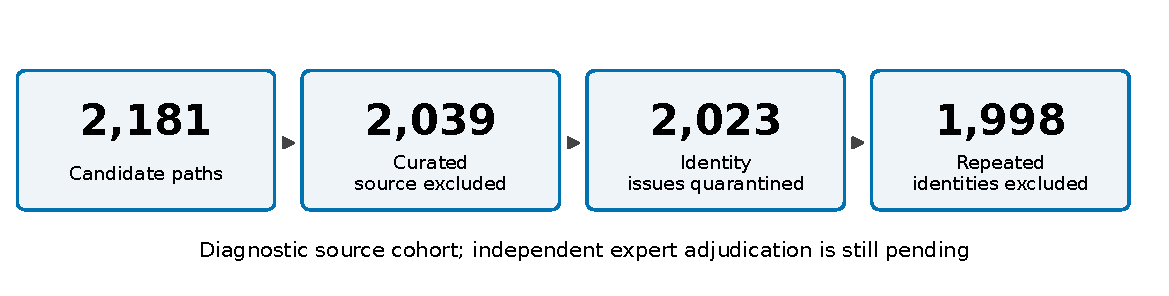
\includegraphics[width=\linewidth,height=0.75\textheight,keepaspectratio]{figureS1.pdf}
\caption{Source-based selection of the diagnostic external cohort. The 1,998 retained files are a provisional population, not an independently verified test. Source exclusions and training restrictions are different decisions. Of 17 originally problematic paths, one is removed by the earlier curated-source exclusion.}\label{fig:S1}
\end{figure}

Direct screening is insufficient for transitive separation. Among the 1,998 retained files, 65 have a direct 0.8 lexical relation to reference data, whereas 186 in 11 proxy components are connected transitively. Retaining the entire diagnostic test and excluding connected historical training components leaves 691 DAppSCAN files, with 23 reentrancy and 18 unchecked proxy positives. Another 350 SolidiFI and 134 SmartBugs files remain, but their different annotation origins cannot be used to conceal the loss of DAppSCAN support in a pooled positive count. DAppSCAN retention changes from 418 at threshold 0.7 to 1,085 at 0.9.

The string-aware scanner changes 92 of 24,131 normalized streams without a scan failure. Fourteen lexical edges disappear at 0.7, none at 0.8 or 0.9, and no training-retention decision changes at those thresholds. Adding 80 equal-address links also changes no partition. These are useful robustness checks for this dataset, rather than evidence that representation choices or deployment provenance are generally unimportant.

The compiler check succeeds for 2,137 of the 2,689 fixed files (79.47\%): 1,807/1,998 external files (90.44\%) and 330/691 training files (47.76\%). Conditioning on attempted compilation gives different figures: 1,807/1,968 (91.82\%) and 330/336 (98.21\%), respectively. We retain the fixed-cohort denominators because input-context failures are part of practical coverage. The 552 other files comprise 385 unavailable inputs or compiler plans and 167 final compiler errors. In particular, 346 training files lack an accepted import context; this does not establish that their sources are invalid. No file is dropped because compilation fails.

Of the 330 successful training files, 101 have no nonempty root bytecode. Interface or abstract-only sources can compile without providing a deployable target. Twenty successes, ten in each cohort, contain unlinked root bytecode. Compilation therefore establishes neither executable-contract coverage nor successful Slither analysis. These results leave the fixed training and external populations unchanged; they do not justify restricting a detector's reported denominator to successful compilations.

For this proposed external evaluation, no Slither corpus analysis, independent human vulnerability assessment or external ML fit or score has been completed. The source, dependency and compilation audits establish specific readiness conditions, while annotation correctness, deployment-family identity and external performance remain separate empirical questions.

\section{Auxiliary representation-based training eligibility}\label{auxiliary-representation-based-training-eligibility}

This calculation uses a fixed provisional candidate cohort as a geometric query set. It measures historical training support after graph exclusion rather than detector performance.

\begingroup
\small
\setlength{\tabcolsep}{4pt}
\setlength{\LTcapwidth}{\linewidth}
\renewcommand{\arraystretch}{1.14}
\begin{longtable}{>{\raggedright\arraybackslash}p{\dimexpr 0.19000\linewidth-2\tabcolsep\relax}>{\raggedright\arraybackslash}p{\dimexpr 0.15000\linewidth-2\tabcolsep\relax}>{\raggedright\arraybackslash}p{\dimexpr 0.19000\linewidth-2\tabcolsep\relax}>{\raggedright\arraybackslash}p{\dimexpr 0.15000\linewidth-2\tabcolsep\relax}>{\raggedright\arraybackslash}p{\dimexpr 0.16000\linewidth-2\tabcolsep\relax}>{\raggedright\arraybackslash}p{\dimexpr 0.16000\linewidth-2\tabcolsep\relax}}
\caption{Representation sensitivity at Jaccard 0.8. All variants retain 24,131 graph nodes and the same 1,998 candidate test files. The largest component is projected onto all 21,457 DAppSCAN files. Training columns concern the historical 6,587-file DAppSCAN population after excluding components touching that fixed candidate test; positive counts are among informative retained files.}\label{tab:S1}\\
\toprule
\textbf{Source representation} & \textbf{Identifiers and numbers} & \textbf{Largest DAppSCAN component} & \textbf{Graph-retained training} & \textbf{Informative retained training} & \textbf{Retained proxy positives, reentrancy / unchecked} \\
\midrule
\endfirsthead
\toprule
\textbf{Source representation} & \textbf{Identifiers and numbers} & \textbf{Largest DAppSCAN component} & \textbf{Graph-retained training} & \textbf{Informative retained training} & \textbf{Retained proxy positives, reentrancy / unchecked} \\
\midrule
\endhead
\midrule
\multicolumn{6}{r}{\footnotesize Continued on next page} \\
\endfoot
\bottomrule
\endlastfoot
Full file & Collapsed & 20,565 (95.84\%) & 712 & 711 & 23 / 18 \\
Full file & Preserved & 18,769 (87.47\%) & 1,504 & 1,502 & 37 / 29 \\
Library/\allowbreak interface declarations masked & Collapsed & 18,745 (87.36\%) & 1,520 & 1,086 & 36 / 25 \\
Library/\allowbreak interface declarations masked & Preserved & 17,177 (80.05\%) & 2,150 & 1,539 & 49 / 36 \\
\end{longtable}
\endgroup

The common empty-input policy changes graph-retained historical DAppSCAN training from 691 to 712 files, of which 711 are informative, before the factorial contrasts. Masking suppresses lexical participation while preserving graph nodes and explicit project/raw-identity relations; graph retention therefore differs from usable lexical support. The new availability-only control in the main text further separates these mechanisms. Indeed, 5,198 and 4,742 unavailable DAppSCAN nodes still belong to the actual masked giant under collapsed and preserved tokens, respectively, through the retained structural relations. The masked giant also changes membership: it loses eight DAppSCAN nodes and gains 25 or 31 relative to the availability-only giant under collapsed or preserved tokens, respectively.

The segmented-mask control preserves Jaccard 0.8 largest-component and candidate-separated training counts in both masked variants, although some component memberships change. With containment, informative training changes from 22 to 41 files for collapsed tokens and from 739 to 740 for preserved tokens.

\subsection{Exact-identity controls on DAppSCAN}\label{exact-identity-controls-on-dappscan}

All four controls construct the graph on the same 21,457 DAppSCAN files. Project relations are retained. The nonempty lexical variants exclude six empty sources from equality links while retaining their vertices.

\begingroup
\small
\setlength{\tabcolsep}{4pt}
\setlength{\LTcapwidth}{\linewidth}
\renewcommand{\arraystretch}{1.14}
\begin{longtable}{>{\raggedright\arraybackslash}p{\dimexpr 0.34000\linewidth-2\tabcolsep\relax}>{\raggedright\arraybackslash}p{\dimexpr 0.33000\linewidth-2\tabcolsep\relax}>{\raggedright\arraybackslash}p{\dimexpr 0.33000\linewidth-2\tabcolsep\relax}}
\caption{Exact-identity controls on the complete DAppSCAN population. Empty lexical sequences have no equality links; all vertices and project relations remain.}\label{tab:S2}\\
\toprule
\textbf{Identity relation combined with project membership} & \textbf{Largest component} & \textbf{Share of DAppSCAN} \\
\midrule
\endfirsthead
\toprule
\textbf{Identity relation combined with project membership} & \textbf{Largest component} & \textbf{Share of DAppSCAN} \\
\midrule
\endhead
\midrule
\multicolumn{3}{r}{\footnotesize Continued on next page} \\
\endfoot
\bottomrule
\endlastfoot
Raw bytes & 3,608 & 16.82\% \\
Exact nontrivia lexeme sequence, preserving all lexemes and boundaries & 10,922 & 50.90\% \\
Exact inherited identifier/number-preserving token stream & 11,172 & 52.07\% \\
Exact inherited normalized token stream, nonempty & 19,298 & 89.94\% \\
\end{longtable}
\endgroup

The strict formatting-only scanner preserves quoted content, punctuation, operators, identifiers and numbers. It records zero scan failures and passes 23 scanner checks, independent union-find reconstruction and three partition-refinement checks. The inherited token-preserving relation omits constructs excluded by its tokenizer and is therefore a different control. Jaccard 1.0 and exact ordered-stream equality yield the same reported largest-component counts in the new controls, which does not imply identical partitions or relation definitions.

\section{Incomplete-label AP calculations}\label{incomplete-label-ap-calculations}

These calculations concern inference with incomplete labels rather than the complete proxy-label evaluations in the main text. Yilmaz and Aslam \cite{yilmaz2008incomplete} develop statistical AP estimates from incomplete relevance judgments; the calculation below distinguishes estimation from logical bounds conditional on fixed known labels.

Before external scoring, we examine a proposed survey-weighted AP percentile procedure on 59 prespecified artificial finite populations and sampling designs. The rescaled bootstrap for stratified sampling without replacement uses the finite-population correction in Section 7.2 of the Household Finance and Consumption Network report \cite{hfcn2023methodological}. Its variance motivation is not an AP coverage guarantee. We enumerate every sample and the finite bootstrap support, keeping interval issuance, coverage conditional on issuance, and the probability of issuing a covering interval separate. No actual external score or expert response enters this diagnostic.

A distinct calculation assumes finite scores for every item and partial labels in \{positive, negative, unknown\}. It gives sharp AP endpoints over all feasible binary completions, treating unsampled and unresolved labels as unknown. These are logical identification bounds, not confidence intervals or survey-weighted estimates. The following subsections specify both calculations, the tied-score dynamic program and their synthetic results. Neither calculation changes the interpretation of the complete proxy labels used in the main manuscript's fixed-test model section or supplies external vulnerability validation.

\subsection{Prespecified interval diagnostic}\label{prespecified-interval-diagnostic}

The main synthetic factorial has 20 items, three designs (simple random sampling of four without replacement; two strata of sizes 16 and 4 with two sampled from each; and census), three score patterns (distinct, tied in groups of five, and all tied), and six positive-label patterns. Two no-positive guards and three 50-item, one-positive examples complete the 59 scenarios. We enumerate all 795,934 sample states, with their design probabilities, rather than approximate the sampling distribution. All scores and labels are artificial.

Survey-weighted AP substitutes design-weighted positive and item totals into the grouped-threshold AP formula. Within stratum \(h\), base weights are \(w_h=N_h/n_h\). Drawing \(m_h=n_h-1\) items with replacement gives multiplicities \(r_{hi}\) and replicate weights

\[
w^*_{hi}=w_h\left(1-\lambda_h+\lambda_h\frac{n_h}{m_h}r_{hi}\right),
\qquad \lambda_h=\sqrt{\frac{m_h(1-n_h/N_h)}{n_h-1}}.
\]

Census weights remain fixed. The finite-correction formula follows \cite{hfcn2023methodological}; no AP coverage theorem is assumed. Exact-bootstrap endpoints use the discrete inverse CDF at 0.025 and 0.975. The production procedure also uses 2,000 replicates with each of three prespecified seeds and its saved quantile convention. All four calculations give the same coverage and mean-width summaries in this grid. Undefined AP is never replaced by zero.

Among the 39 positive-population noncensus scenarios, conditional coverage of nominal 95\% intervals ranges from 22.22\% to 100\%; 16 scenarios fall below 95\%. These counts characterize the chosen grid, not the prevalence of failures elsewhere. All 18 positive census controls give exact point intervals; both no-positive guards retain undefined AP.

One example is countable directly. A single positive belongs to the highest tied group of five among 20 items, giving true AP 0.2. An SRS of four includes it with probability 20\%. Conditional on inclusion, the other three items have \(\binom{19}{3}=969\) possible selections. In \(\binom{15}{3}=455\), no other highest-group item is sampled; every positive-weight replicate then has AP one, and the interval is the incorrect \([1,1]\). The other 514 selections cover, giving conditional coverage \(514/969=53.04\%\), and a 10.61\% probability of issuing a covering interval. An unequal-strata example with two positives gives 22.22\% conditional coverage. More bootstrap draws cannot repair the first example's loss of ranking information.

\subsection{Sharp completion bounds and exact verification}\label{sharp-completion-bounds-and-exact-verification}

For a declared population of \(N\) items with finite scores, sort its \(G\) equal-score groups from highest to lowest. Group \(g\) has \(a_g\) known positives and \(u_g\) unknown labels; \(N_g\) and \(A_g\) are cumulative item and known-positive counts. Choosing \(z_g\in\{0,\ldots,u_g\}\) unknown positives gives group count \(p_g=a_g+z_g\), cumulative positives \(T_g\), and total positives \(P\). Grouped-threshold AP, with ties retained, is

\[
\operatorname{AP}=\frac{1}{P}\sum_g\frac{p_gT_g}{N_g},\qquad P>0.
\]

A dynamic program keeps the two extreme numerators for each cumulative unknown-positive count \(t\):

\[
F_g^{\min/\max}(t)=\min/\max_z\left\{
F_{g-1}^{\min/\max}(t-z)+\frac{(a_g+z)(A_g+t)}{N_g}
\right\},\qquad F_0(0)=0.
\]

The optimization uses feasible preceding states and \(0\le z\le u_g\). Every prefix decomposes into one preceding count and one current count; subsequent terms depend on the earlier assignment only through its cumulative positives. Thus retaining these extrema loses no optimum. At the final group, division by the fixed denominator \(P=A_G+t>0\), followed by optimization across terminal states, gives attainable global endpoints. Saved choices reconstruct feasible label completions at both bounds. A greedy earliest/latest assignment of unknown positives is not generally optimal when scores tie.

The implementation scales terms by \(\operatorname{lcm}(N_1,\ldots,N_G)\), uses integer transitions and returns rational endpoints. It needs \(O(Nm)\) transitions for \(m>0\) unknown labels, plus sorting; the bit cost depends on the scaling integer. A possible all-negative completion is reported separately as undefined. A point AP is returned only if every feasible completion identifies the same defined value. The interval is an envelope: not every interior real value must be attainable. It carries no sampling probability or 95\% interpretation, and makes no claim of mathematical priority.

Exhaustive validation through six items covers every ordered tie pattern and partial-label vector: 27,993 cases and 149,796 binary completions. An independent exact threshold formula agrees with every fixed-total and global endpoint, including their attaining completions. The artifact includes the proof, input restrictions, executable implementation, validation records and complete synthetic interval grid. These calculations do not evaluate the actual external cohort.

The artificial interval diagnostic neither estimates coverage for the planned review of 180 file/class cases from the 1,998-file external population nor invalidates every bootstrap approach. Completion bounds condition on correct known labels and finite scores for the declared population. They exclude reviewer error, training variability and unseen families. If a method fails to score an intended file, a success-only bound concerns a changed population. Separate AP bounds give a conservative, generally nonsharp difference envelope rather than a confidence statement about superiority.

\section{Supplementary model-linkage diagnostics}\label{supplementary-model-linkage-diagnostics}

The original historical experiment completed 320 main-panel and 40 seed-panel logical evaluations, with complete test scores, no failed fit and no convergence warning. Its four raw-LR draw-zero score vectors reproduce the original pilot exactly. The graph-model audit below concerns those saved predictions. For the 1,082-file historical test, all files are connected to training under C in all 80 original historical draw/regime cells. The exclusive categories use direct project-or-clone relations first, then B-transitive-only paths, then newly connected C paths, and finally C-disconnected status. Direct flags are also retained separately.

\begingroup
\small
\setlength{\tabcolsep}{4pt}
\setlength{\LTcapwidth}{\linewidth}
\renewcommand{\arraystretch}{1.14}
\begin{longtable}{>{\raggedright\arraybackslash}p{\dimexpr 0.23000\linewidth-2\tabcolsep\relax}>{\raggedright\arraybackslash}p{\dimexpr 0.23000\linewidth-2\tabcolsep\relax}>{\raggedright\arraybackslash}p{\dimexpr 0.27000\linewidth-2\tabcolsep\relax}>{\raggedright\arraybackslash}p{\dimexpr 0.27000\linewidth-2\tabcolsep\relax}}
\caption{Connectivity of the original historical test to its historical training memberships. Counts are ranges across the twenty draws in each regime.}\label{tab:S3}\\
\toprule
\textbf{Historical training regime} & \textbf{Direct-union test files across draws} & \textbf{B-transitive-only files} & \textbf{Reentrancy positives in direct / transitive groups} \\
\midrule
\endfirsthead
\toprule
\textbf{Historical training regime} & \textbf{Direct-union test files across draws} & \textbf{B-transitive-only files} & \textbf{Reentrancy positives in direct / transitive groups} \\
\midrule
\endhead
\midrule
\multicolumn{4}{r}{\footnotesize Continued on next page} \\
\endfoot
\bottomrule
\endlastfoot
Unrestricted & 1,001--1,049 & 33--81 & 17--20 / 1--4 \\
Project-disjoint & 66--78 & 1,004--1,016 & 0 / 21 \\
Clone-disjoint & 978--1,022 & 60--104 & 17--20 / 1--4 \\
Joint-disjoint & 0 & 0 & All 21 occur in the newly C-connected group \\
\end{longtable}
\endgroup

For project-disjoint training the direct-clone subgroup has zero positives, so AP is undefined; the small transitive-only groups of the unrestricted and clone regimes contain only one to four positives. These subgroup populations differ in both size and composition. Review-yield contributions retain the original full-test budgets and sum to the original total, including expected tie handling. Every full-test AP reproduces its stored value within 1e−14. These checks validate the descriptive decomposition without creating an unconnected expanded-graph comparison group.

\subsection{Precursor matched B--C policy experiment}\label{precursor-matched-bc-policy-experiment}

The precursor experiment uses the unchanged 1,082-file test and the same historical model configurations. B supplies five distinct class-stratified 708-file/24-positive draws; C supplies its one complete 708-file/24-positive pool. LR uses seed zero and tree methods use paired seeds zero through four. There are 72 distinct physical fits and 120 logical evaluations, with 12 C fits reused across draw indices. The run has zero failed fits and zero convergence warnings. Thirty nonfatal LightGBM feature-name warnings are preserved in the execution records; none were filtered from the audit trail.

A separate arithmetic implementation independently recomputed all 120 AP values and all 360 budget-yield values. Every comparison passed. Complete paired outcomes, training memberships, source hashes, plans and warning records are retained under \nolinkurl{revision2/model_link/expanded_contrast_20261028_v1/}. Table S4 reports its B-minus-C AP contrasts. The repeated use of the C pool and test means that 25 tree comparisons are not 25 independent model families or test replications.

\begingroup
\small
\setlength{\tabcolsep}{4pt}
\setlength{\LTcapwidth}{\linewidth}
\renewcommand{\arraystretch}{1.14}
\begin{longtable}{>{\raggedright\arraybackslash}p{\dimexpr 0.21000\linewidth-2\tabcolsep\relax}>{\raggedright\arraybackslash}p{\dimexpr 0.19750\linewidth-2\tabcolsep\relax}>{\raggedright\arraybackslash}p{\dimexpr 0.19750\linewidth-2\tabcolsep\relax}>{\raggedright\arraybackslash}p{\dimexpr 0.19750\linewidth-2\tabcolsep\relax}>{\raggedright\arraybackslash}p{\dimexpr 0.19750\linewidth-2\tabcolsep\relax}}
\caption{AP in the precursor 1,082-file matched experiment. Both training policies retain 708 files and 24 positives. Means and extrema describe five training draws, with one LR seed or five paired tree seeds. They are not independent-test confidence intervals.}\label{tab:S4}\\
\toprule
\textbf{Method} & \textbf{B mean AP} & \textbf{C mean AP} & \textbf{Mean B−C} & \textbf{B−C range} \\
\midrule
\endfirsthead
\toprule
\textbf{Method} & \textbf{B mean AP} & \textbf{C mean AP} & \textbf{Mean B−C} & \textbf{B−C range} \\
\midrule
\endhead
\midrule
\multicolumn{5}{r}{\footnotesize Continued on next page} \\
\endfoot
\bottomrule
\endlastfoot
Raw-token LR & 0.034481 & 0.028383 & +0.006098 & {[}-0.005448, +0.018700{]} \\
Normalized-token LR & 0.049071 & 0.035399 & +0.013672 & {[}+0.000584, +0.029484{]} \\
Pattern random forest & 0.078779 & 0.052509 & +0.026270 & {[}-0.003022, +0.055742{]} \\
Pattern LightGBM & 0.076546 & 0.044357 & +0.032189 & {[}-0.001814, +0.093872{]} \\
\end{longtable}
\endgroup

\begingroup
\small
\setlength{\tabcolsep}{4pt}
\setlength{\LTcapwidth}{\linewidth}
\renewcommand{\arraystretch}{1.14}
\begin{longtable}{>{\raggedright\arraybackslash}p{\dimexpr 0.21000\linewidth-2\tabcolsep\relax}>{\raggedright\arraybackslash}p{\dimexpr 0.19750\linewidth-2\tabcolsep\relax}>{\raggedright\arraybackslash}p{\dimexpr 0.19750\linewidth-2\tabcolsep\relax}>{\raggedright\arraybackslash}p{\dimexpr 0.19750\linewidth-2\tabcolsep\relax}>{\raggedright\arraybackslash}p{\dimexpr 0.19750\linewidth-2\tabcolsep\relax}}
\caption{Complete review-budget results for the precursor matched experiment. Cells give mean proxy-positive findings, using expected counts at boundary ties. Uniform random ranking has expected yields 1.0481, 2.0961 and 4.1922 at budgets 54, 108 and 216. The same historically inspected labels are used throughout.}\label{tab:S5}\\
\toprule
\textbf{Method} & \textbf{Reviews} & \textbf{B findings} & \textbf{C findings} & \textbf{Mean B−C} \\
\midrule
\endfirsthead
\toprule
\textbf{Method} & \textbf{Reviews} & \textbf{B findings} & \textbf{C findings} & \textbf{Mean B−C} \\
\midrule
\endhead
\midrule
\multicolumn{5}{r}{\footnotesize Continued on next page} \\
\endfoot
\bottomrule
\endlastfoot
Raw-token LR & 54 & 2.0000 & 2.0000 & +0.0000 \\
Raw-token LR & 108 & 3.4000 & 4.0000 & -0.6000 \\
Raw-token LR & 216 & 4.8000 & 4.0000 & +0.8000 \\
Normalized-token LR & 54 & 2.8000 & 4.0000 & -1.2000 \\
Normalized-token LR & 108 & 5.6000 & 5.0000 & +0.6000 \\
Normalized-token LR & 216 & 7.6000 & 5.0000 & +2.6000 \\
Pattern random forest & 54 & 4.5467 & 1.8000 & +2.7467 \\
Pattern random forest & 108 & 8.4225 & 6.2229 & +2.1997 \\
Pattern random forest & 216 & 13.0480 & 11.8000 & +1.2480 \\
Pattern LightGBM & 54 & 3.8000 & 2.0000 & +1.8000 \\
Pattern LightGBM & 108 & 7.6400 & 4.2000 & +3.4400 \\
Pattern LightGBM & 216 & 11.4000 & 8.8000 & +2.6000 \\
\end{longtable}
\endgroup

Raw LR has identical yields at 54 reviews, lower mean yield under B at 108, and higher yield under B at 216. Normalized LR favors C at 54 reviews and B at the larger budgets. The tree methods have higher mean B yield at all three budgets, although individual paired comparisons can reverse. Thus the precursor's mean AP ordering does not imply a uniform workload ordering.

\subsection{Full-giant comparison and complete review budgets}\label{full-giant-comparison-and-complete-review-budgets}

The expanded experiment scores 5,408 files with 83 positives. All 852 planned fits completed with complete score vectors, no failed fit and no convergence warning. The execution records retain 355 LightGBM feature-name warnings. An independent replay checked all 852 score vectors, 10,224 frame-level AP calculations and their review-budget quantities; separate aggregation checks reproduce the composition distributions and retention summaries. The largest per-fit AP discrepancy in that independent replay was \(5.55\times10^{-17}\); per-fit review yields and empirical distribution counts agree exactly.

\begingroup
\small
\setlength{\tabcolsep}{4pt}
\setlength{\LTcapwidth}{\linewidth}
\renewcommand{\arraystretch}{1.14}
\begin{longtable}{>{\raggedright\arraybackslash}p{\dimexpr 0.21000\linewidth-2\tabcolsep\relax}>{\raggedright\arraybackslash}p{\dimexpr 0.19750\linewidth-2\tabcolsep\relax}>{\raggedright\arraybackslash}p{\dimexpr 0.19750\linewidth-2\tabcolsep\relax}>{\raggedright\arraybackslash}p{\dimexpr 0.19750\linewidth-2\tabcolsep\relax}>{\raggedright\arraybackslash}p{\dimexpr 0.19750\linewidth-2\tabcolsep\relax}}
\caption{Complete review-budget results for the full-giant comparison. B means average 50 compositions; tree review-yield values are averaged over seeds within each composition. C uses its complete pool. At budgets 270, 540 and 1,081, random ranking has expected yields 4.1439, 8.2877 and 16.5908. Boundary ties use expected findings within the tied block.}\label{tab:S6}\\
\toprule
\textbf{Method} & \textbf{Reviews} & \textbf{B findings} & \textbf{C findings} & \textbf{Mean B−C} \\
\midrule
\endfirsthead
\toprule
\textbf{Method} & \textbf{Reviews} & \textbf{B findings} & \textbf{C findings} & \textbf{Mean B−C} \\
\midrule
\endhead
\midrule
\multicolumn{5}{r}{\footnotesize Continued on next page} \\
\endfoot
\bottomrule
\endlastfoot
Raw-token LR & 270 & 4.0600 & 4.0000 & +0.0600 \\
Raw-token LR & 540 & 7.2600 & 4.0000 & +3.2600 \\
Raw-token LR & 1,081 & 13.2000 & 9.0000 & +4.2000 \\
Normalized-token LR & 270 & 8.3200 & 10.0000 & -1.6800 \\
Normalized-token LR & 540 & 16.9000 & 15.0000 & +1.9000 \\
Normalized-token LR & 1,081 & 30.9400 & 25.0000 & +5.9400 \\
Pattern random forest & 270 & 16.1006 & 10.4500 & +5.6506 \\
Pattern random forest & 540 & 29.7823 & 20.3333 & +9.4490 \\
Pattern random forest & 1,081 & 53.9137 & 42.4505 & +11.4632 \\
Pattern LightGBM & 270 & 13.3020 & 9.2000 & +4.1020 \\
Pattern LightGBM & 540 & 25.1520 & 15.2000 & +9.9520 \\
Pattern LightGBM & 1,081 & 45.4200 & 35.2000 & +10.2200 \\
\end{longtable}
\endgroup

Raw LR has mean yields below the random references under both policies at every budget. Normalized LR favors C at the smallest budget and B at the other two. Both tree methods favor B in all three mean comparisons, but individual composition contrasts include reversals. AP and review yield therefore describe different aspects of the same rankings.

\subsection{Linked-file retention}\label{linked-file-retention}

The zero-linked endpoint is the complete C pool. The other levels use five nested compositions, with tree AP and review-yield values averaged over five paired seeds. Each training set contains 708 files and 24 positives; the linked-positive counts are 0, 2, 4, 5 and 7. Full linked retention means keeping all 471 newly connected files, or 66.53\% of training. Every positive retention level already makes every test file C-connected to training.

\begingroup
\small
\setlength{\tabcolsep}{4pt}
\setlength{\LTcapwidth}{\linewidth}
\renewcommand{\arraystretch}{1.14}
\begin{longtable}{>{\raggedright\arraybackslash}p{\dimexpr 0.21000\linewidth-2\tabcolsep\relax}>{\raggedright\arraybackslash}p{\dimexpr 0.19750\linewidth-2\tabcolsep\relax}>{\raggedright\arraybackslash}p{\dimexpr 0.19750\linewidth-2\tabcolsep\relax}>{\raggedright\arraybackslash}p{\dimexpr 0.19750\linewidth-2\tabcolsep\relax}>{\raggedright\arraybackslash}p{\dimexpr 0.19750\linewidth-2\tabcolsep\relax}}
\caption{Mean AP by number of newly connected training files retained. Means are over the five composition rankings, after seed averaging for trees. The zero-linked C endpoint is reused. Monotonicity refers only to the mean series, not every fitted model.}\label{tab:S7}\\
\toprule
\textbf{Linked files retained} & \textbf{Raw-token LR} & \textbf{Normalized-token LR} & \textbf{Random forest} & \textbf{LightGBM} \\
\midrule
\endfirsthead
\toprule
\textbf{Linked files retained} & \textbf{Raw-token LR} & \textbf{Normalized-token LR} & \textbf{Random forest} & \textbf{LightGBM} \\
\midrule
\endhead
\midrule
\multicolumn{5}{r}{\footnotesize Continued on next page} \\
\endfoot
\bottomrule
\endlastfoot
0 & 0.012256 & 0.022531 & 0.041768 & 0.040843 \\
118 & 0.012753 & 0.025075 & 0.046604 & 0.038195 \\
236 & 0.016599 & 0.027405 & 0.055039 & 0.045370 \\
353 & 0.015170 & 0.031184 & 0.058934 & 0.052820 \\
471 & 0.016113 & 0.032228 & 0.070310 & 0.062354 \\
\end{longtable}
\endgroup

\begin{figure}[htbp]
\centering
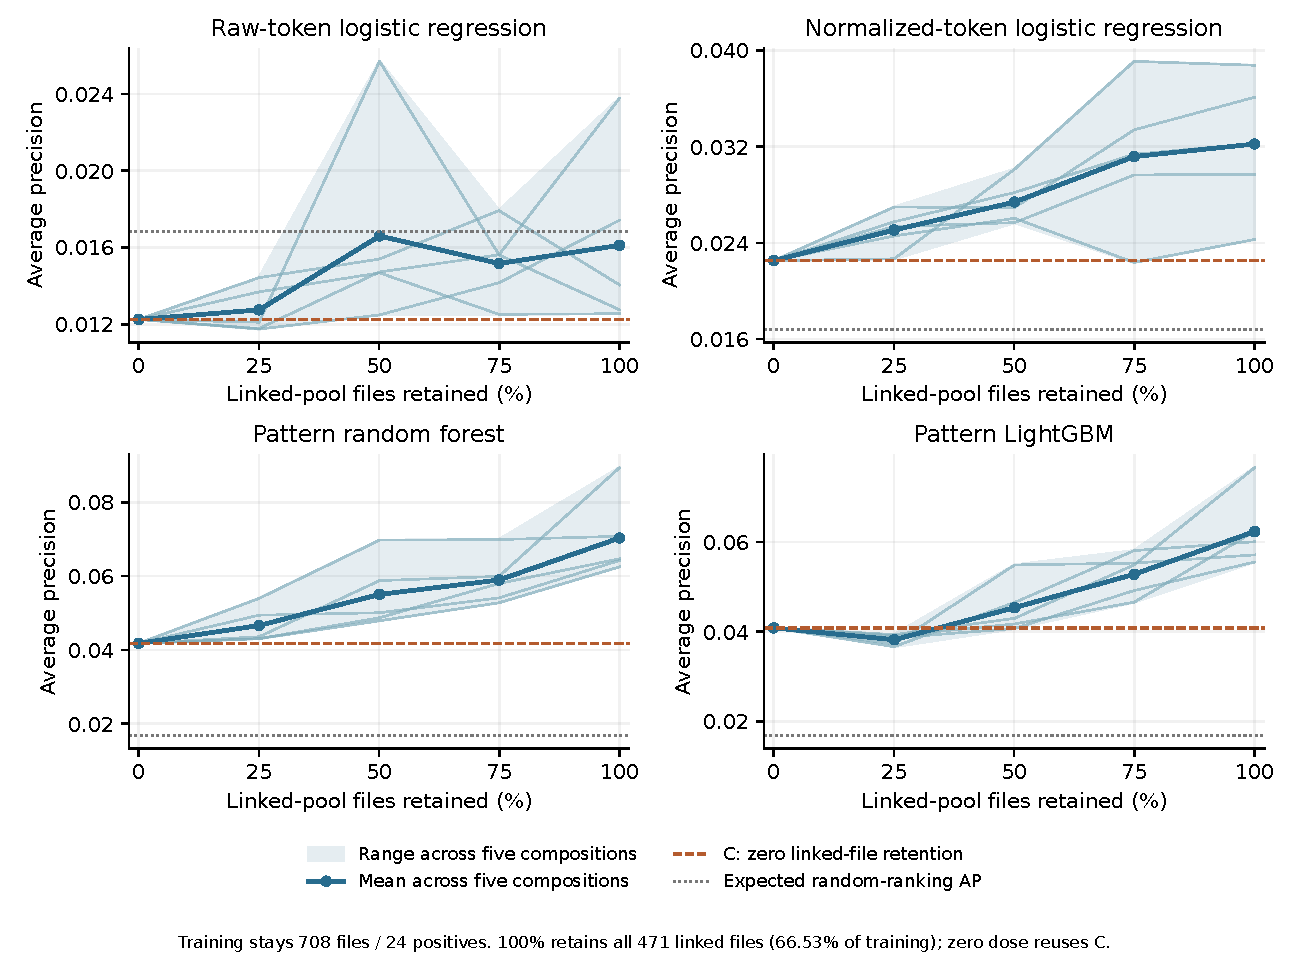
\includegraphics[width=\linewidth,height=0.75\textheight,keepaspectratio]{figureS2.pdf}
\caption{AP across the linked-file retention levels. Thin blue lines show five nested compositions, the bold line their mean, and shading their observed range after averaging AP over tree seeds. Orange marks the zero-retention endpoint with one reused C membership; grey gives expected random-ranking AP. Training size and positive count remain 708 and 24. The 100\% endpoint retains all 471 linked files, or 66.53\% of training. Ranges are descriptive, not confidence intervals.}\label{fig:S2}
\end{figure}

\clearpage
\begin{landscape}
\begin{figure}[p]
\centering
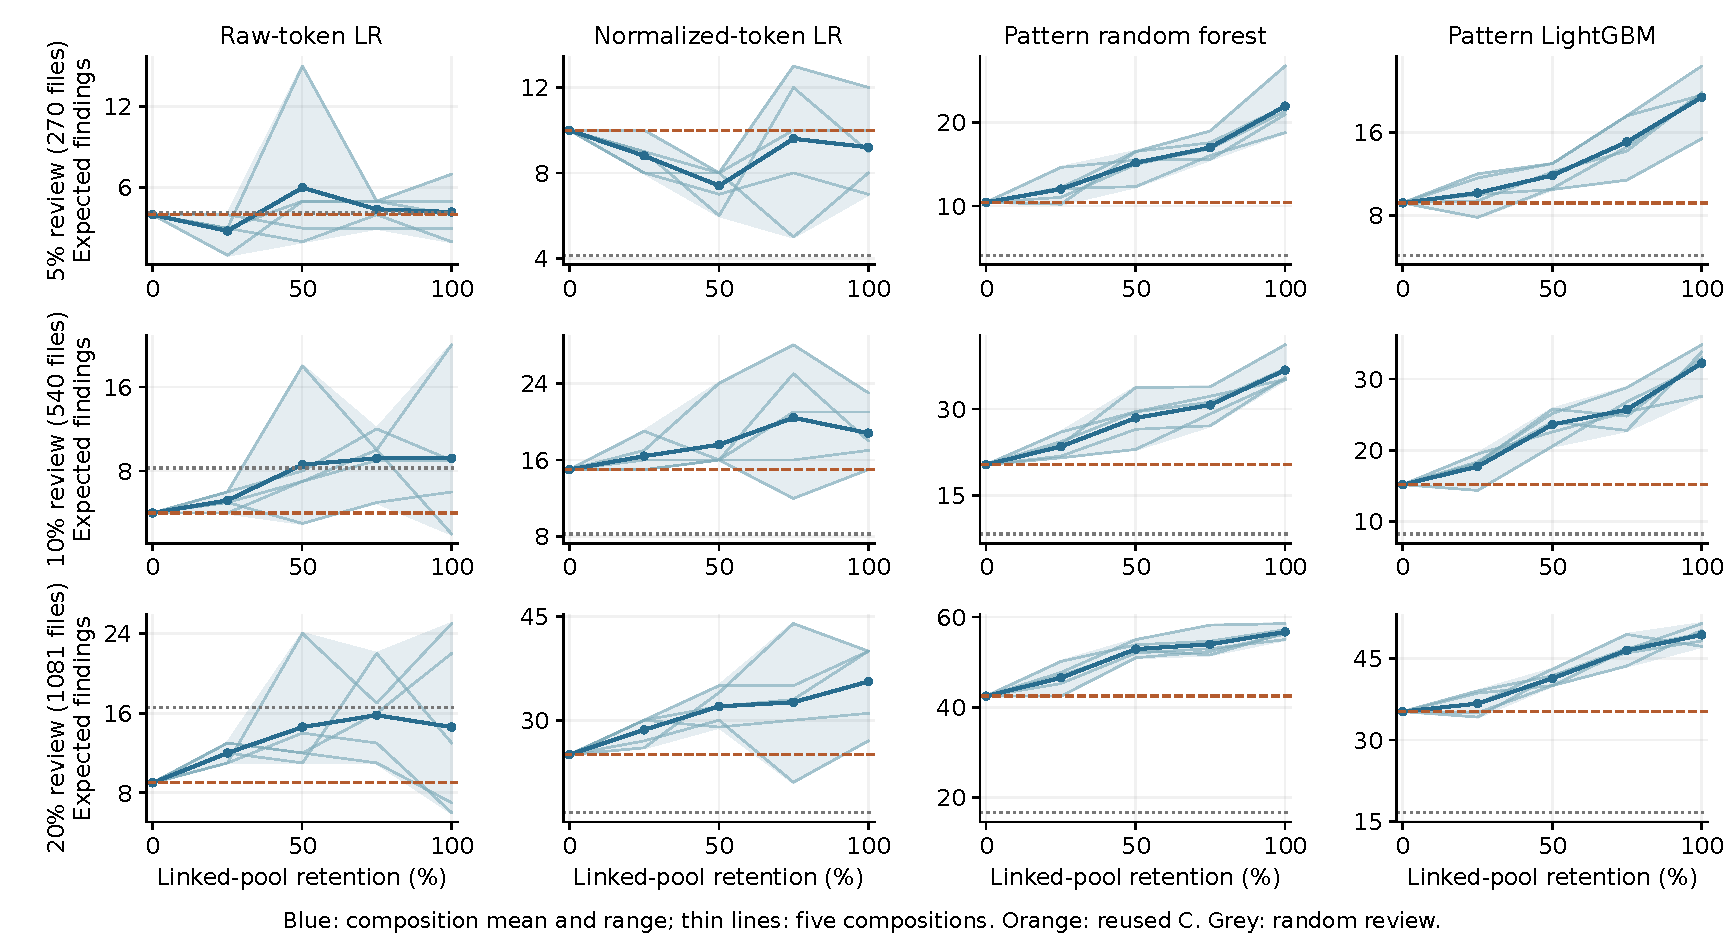
\includegraphics[width=235mm,height=135mm,keepaspectratio]{figureS3.pdf}
\caption{Expected findings at 270, 540 and 1,081 reviews for all four methods on the fixed 5,408-file, 83-positive test. Thin blue lines, bold means and shaded ranges summarize five retention compositions after averaging review-yield values over tree seeds. Orange dashes mark reused C; grey dots mark random review. Boundary ties use uniform-order expectations. Training remains 708 files with 24 positives; 100\% retains all 471 linked files. Shading is not a confidence interval.}\label{fig:S3}
\end{figure}
\end{landscape}
\clearpage

\subsection{Sensitivity to overlapping test slices}\label{sensitivity-to-overlapping-test-slices}

The ten previously defined label-blind slices each contain 1,062 files and 13--21 positives. Their pairwise intersections range from 184 to 231 files; their union covers 4,806 of the 5,408 giant files. All slices induce the same B and C training pools. Table S8 retains every mean contrast, including negative ones. Their overlap and common graph component preclude interpretation as ten independent families.

\begingroup
\small
\setlength{\tabcolsep}{4pt}
\setlength{\LTcapwidth}{\linewidth}
\renewcommand{\arraystretch}{1.14}
\begin{longtable}{>{\raggedright\arraybackslash}p{\dimexpr 0.11000\linewidth-2\tabcolsep\relax}>{\raggedright\arraybackslash}p{\dimexpr 0.14000\linewidth-2\tabcolsep\relax}>{\raggedright\arraybackslash}p{\dimexpr 0.18000\linewidth-2\tabcolsep\relax}>{\raggedright\arraybackslash}p{\dimexpr 0.21000\linewidth-2\tabcolsep\relax}>{\raggedright\arraybackslash}p{\dimexpr 0.18000\linewidth-2\tabcolsep\relax}>{\raggedright\arraybackslash}p{\dimexpr 0.18000\linewidth-2\tabcolsep\relax}}
\caption{Mean B-minus-C AP on the ten internal slices. B has 50 compositions; tree seeds are averaged within composition. The test identifiers correspond to the frozen path-hash selections.}\label{tab:S8}\\
\toprule
\textbf{Test seed} & \textbf{Positives} & \textbf{Raw-token LR} & \textbf{Normalized-token LR} & \textbf{Random forest} & \textbf{LightGBM} \\
\midrule
\endfirsthead
\toprule
\textbf{Test seed} & \textbf{Positives} & \textbf{Raw-token LR} & \textbf{Normalized-token LR} & \textbf{Random forest} & \textbf{LightGBM} \\
\midrule
\endhead
\midrule
\multicolumn{6}{r}{\footnotesize Continued on next page} \\
\endfoot
\bottomrule
\endlastfoot
1301 & 19 & +0.004879 & +0.019366 & +0.053688 & +0.047157 \\
1302 & 19 & +0.000782 & +0.002232 & -0.033451 & +0.010077 \\
1303 & 21 & -0.000783 & +0.011599 & +0.037026 & +0.015102 \\
1304 & 13 & +0.008090 & +0.015613 & +0.036776 & +0.000179 \\
1305 & 18 & +0.003279 & +0.011396 & +0.055003 & -0.009566 \\
1306 & 13 & +0.010837 & +0.001898 & +0.006945 & +0.007952 \\
1307 & 13 & +0.004998 & +0.027234 & +0.026417 & +0.030260 \\
1308 & 15 & +0.010697 & +0.016367 & +0.009255 & +0.005350 \\
1309 & 19 & +0.001644 & +0.004851 & +0.035475 & +0.022494 \\
1310 & 16 & -0.001970 & -0.010135 & +0.020429 & +0.031844 \\
\end{longtable}
\endgroup

Mean contrasts are positive in eight of ten slices for raw LR and nine for each other method. Random forest has a negative contrast on seed 1302, LightGBM on 1305, normalized LR on 1310, and raw LR on 1303 and 1310. On the original 1,082-file test, the enlarged 50-draw raw-LR comparison has B mean AP 0.032541 and C AP 0.028383, but only 28 positive and 22 negative composition differences; C is at the empirical 44th percentile. This precursor sensitivity is reported alongside the full-giant result.

\subsection{Composition associations within the ordinary B draws}\label{composition-associations-within-the-ordinary-b-draws}

The 50 ordinary B draws contain 269--299 newly connected training files (mean 282.48), including 3--7 linked positives (mean 5.34). These counts vary over a much narrower range than the retention experiment. Table S9 reports descriptive Pearson correlations with AP on the full giant. Total training size and total positive count remain fixed. The correlations describe which examples were selected; no causal effect or p-value is inferred.

\begingroup
\small
\setlength{\tabcolsep}{4pt}
\setlength{\LTcapwidth}{\linewidth}
\renewcommand{\arraystretch}{1.14}
\begin{longtable}{>{\raggedright\arraybackslash}p{\dimexpr 0.34000\linewidth-2\tabcolsep\relax}>{\raggedright\arraybackslash}p{\dimexpr 0.33000\linewidth-2\tabcolsep\relax}>{\raggedright\arraybackslash}p{\dimexpr 0.33000\linewidth-2\tabcolsep\relax}}
\caption{Associations between selected linked support and AP across the 50 B compositions. Tree AP is averaged over five seeds before calculating correlations.}\label{tab:S9}\\
\toprule
\textbf{Method} & \textbf{Linked-file count versus AP} & \textbf{Linked-positive count versus AP} \\
\midrule
\endfirsthead
\toprule
\textbf{Method} & \textbf{Linked-file count versus AP} & \textbf{Linked-positive count versus AP} \\
\midrule
\endhead
\midrule
\multicolumn{3}{r}{\footnotesize Continued on next page} \\
\endfoot
\bottomrule
\endlastfoot
Raw-token LR & -0.054 & -0.046 \\
Normalized-token LR & -0.070 & +0.217 \\
Pattern random forest & +0.019 & +0.540 \\
Pattern LightGBM & +0.156 & +0.424 \\
\end{longtable}
\endgroup

\section{Reproducibility and archive lineage}\label{reproducibility-and-archive-lineage}

The \href{https://github.com/KuznetsovKarazin/blockchain-detector-eval/releases/tag/article1-r5-2026-10-29}{article replication release}, tagged \texttt{article1-r5-2026-10-29}, combines versioned code and manifests with the asset \nolinkurl{Article_1_R5_Derived_Evidence_2026-10-29.zip}. The full reproducibility artifact is archived at \href{https://doi.org/10.5281/zenodo.23750089}{10.5281/zenodo.23750089}. The supplied retrieval script verifies its byte length, SHA-256 and member hashes, then restores the recorded paths. Table S10 distinguishes inspecting outputs, recomputing metrics and refitting models.

\begingroup
\small
\setlength{\tabcolsep}{4pt}
\setlength{\LTcapwidth}{\linewidth}
\renewcommand{\arraystretch}{1.14}
\begin{longtable}{>{\raggedright\arraybackslash}p{\dimexpr 0.27000\linewidth-2\tabcolsep\relax}>{\raggedright\arraybackslash}p{\dimexpr 0.32000\linewidth-2\tabcolsep\relax}>{\raggedright\arraybackslash}p{\dimexpr 0.41000\linewidth-2\tabcolsep\relax}}
\caption{Reproduction scenarios and input requirements. Source-dependent scenarios require pinned upstream sources or annotations in addition to the release files.}\label{tab:S10}\\
\toprule
\textbf{Reproduction scenario} & \textbf{Released evidence} & \textbf{Additional inputs and verification scope} \\
\midrule
\endfirsthead
\toprule
\textbf{Reproduction scenario} & \textbf{Released evidence} & \textbf{Additional inputs and verification scope} \\
\midrule
\endhead
\midrule
\multicolumn{3}{r}{\footnotesize Continued on next page} \\
\endfoot
\bottomrule
\endlastfoot
Inspect graph and model summaries & Tables, configurations, manifests, predictions and execution records & No refitting is implied by inspecting stored results \\
Recompute baseline components & Complete baseline nodes and edges with reconstruction code & Pinned annotations for label aggregates; component checks are separate from model fitting \\
Recompute fixed-test and coverage controls & Original compressed memberships, graph files and control definitions & Isolated graph replays cover label-blind tests and project-prefix selections \\
Recompute representation controls & Original membership archives, canonical replacement edges and source-hash records & Pinned source acquisition for lexical reconstruction; replacement lineage is preserved \\
Recompute historical model metrics & Saved score vectors, training memberships and configurations & Restore exact proxy labels from the pinned annotations; arithmetic checks do not refit models \\
Refit the expanded-exclusion and retention models & Frozen plans, memberships, code and runtime versions & Verified sources, annotations and numerical environment; use a separate output directory \\
Repeat incomplete-label AP calculations & Code, synthetic inputs, exact validation and interval-grid results & Numerical environment; no human judgments are required for the synthetic calculations \\
Perform external detector evaluation & Cohort inventory, source reconciliation and compiler audit & Independent vulnerability assessment and subsequent external scoring remain unperformed \\
\end{longtable}
\endgroup

Twenty-three original gzip archives match their recorded historical Git blob identities and internal checksums. Six original representation-edge NPZ archives remain lost. Six canonical NPZ replacements reproduce 120 saved partitions and 20 tables, while six associated membership archives retain their original hashes. This validates the reproduced partition quantities; the original complete edge lists were not recovered. New edge-level analyses record the replacement archive used.

All 21,457 DAppSCAN Solidity files (107,970,249 bytes) and 948 annotation files were verified against frozen hashes at commit \nolinkurl{66a56619c44770e05c2db600fa6468115ff0dcd5}. The acquisition script retrieves the required source and annotation directories. Public inventory rows omit third-party labels; the supplied materializer reconstructs and verifies the exact analysis labels and memberships from the pinned annotations. Other pinned corpora remain distinct upstream inputs.

Seven graph scenarios were independently replayed in an isolated copy of the proposed public release: label-blind tests, project-prefix controls, metadata controls, paired representation controls, strict identity controls, common-informative denominators and structural baselines. Source-dependent checks used the verified pinned DAppSCAN snapshot rather than another network download. These checks cover the release candidate and its stated inputs; they are not a claim of a fresh remote checkout after publication. The precursor model audit independently recomputed 480 AP and review-yield quantities, with a maximum discrepancy of \(1.78\times10^{-15}\). The expanded-model verification is reported with its results in Supplement S4.

\section{Additional implementation and sensitivity detail}\label{additional-implementation-and-sensitivity-detail}

Each minimum-added-vertex path from a newly joined historical component to the original giant requires one or two vertices added when expanding B to C. The unions of the selected paths contain 28 and 29 added vertices for tests 2 and 4, respectively, and suffice to connect all 28 and 29 affected historical components. Each path minimizes its own number of added vertices. Their union is a constructive sufficient set, not a globally minimum connector set or evidence that each selected bridge is uniquely necessary.

The highest-impact project bridge is supported by Tenderize's \texttt{Faucet.sol} and Livepeer's \texttt{LivepeerTokenFaucet.sol} at Jaccard 0.804878; neither witness declares a library or interface. A second bridge joins PieDAO's \texttt{IAToken.sol} and Fei's \nolinkurl{IFeiRewardsDistributor.sol} at 0.809524; both declare interfaces, and the smaller side contains 36 files. These deliberately selected witnesses illustrate heterogeneous connectors. They do not estimate the prevalence of semantic libraries or prove that an individual witness file is indispensable.

Containment produces larger components than Jaccard under every variant at 0.8: 21,454, 20,824, 21,430 and 19,336 DAppSCAN files for full collapsed, full preserved, masked collapsed and masked preserved representations, respectively. Its ability to connect a small representation to a much larger file therefore does not resolve concentration here. It changes which reuse patterns count as dependencies and can make transitive exclusion more restrictive.

A separately frozen segmented-shingle control preserves the main Jaccard 0.8 largest-component counts while preventing shingles from spanning removed declarations. Some memberships change, so equal summary counts do not imply partition invariance; the auxiliary training-support results are retained in Supplement S2.

Historical source-cap detail: The historical population contains 6,587 DAppSCAN files and all 493 reference files, totaling 7,080. The adapter retains every DAppSCAN file linked to a source-annotation record, including records for weaknesses outside the selected classes. This gives 948 metadata-linked files. It then retains at most 20 other files per project directory. Project directories and source paths are sorted; a single Python \texttt{random.Random(0)} generator shuffles each directory's unannotated list before truncation. The result adds 5,639 files without annotation records. The cap was a computational choice intended to prevent large repositories from dominating; it is label-informed and is not a probability sample of the full corpus. The uncapped inventory contains the same 948 metadata-linked files and 20,509 others, across 608 observed project-directory groups.

Historical pattern-feature detail: The pattern vector includes 38 counts of calls, checks, authorization, arithmetic, state and control-flow constructs, normalized per 100 nonempty source lines; a call-before-write heuristic; a parsed compiler-version value and pre-0.8 indicator; and log-transformed line and function counts. These are lexical heuristics, not formal vulnerability predicates. Vectorizers and scalers are fitted on training data only. The model feature code remains historical, including its legacy comment removal, so a graph-normalization sensitivity does not silently change the model experiment.

Random AP expectation derivation: To see this, expand AP as \(K^{-1}\sum_r I_r(\sum_{j\le r}I_j)/r\), using \(\mathbb E I_r=K/N\) and \(\mathbb E I_rI_j=K(K-1)/(N(N-1))\) for distinct positions.
\FloatBarrier
\bibliographystyle{elsarticle-num}
\bibliography{references}
\end{document}
